\documentclass{article}
\usepackage[T1]{fontenc}
\usepackage{lmodern}
\usepackage{graphicx}
\usepackage{amsmath,amssymb}
\usepackage[a4paper,margin=2cm]{geometry}
\usepackage[absolute,overlay]{textpos}
\setlength{\TPHorizModule}{1mm}
\setlength{\TPVertModule}{1mm}
\usepackage[indonesian]{babel}
\usepackage{hyperref}
\setlength{\emergencystretch}{2em}
% unit: Halaman 49

\begin{document}

% === Halaman 49 (python/native) ===

Old Cryptography

• Ancient cryptography atau classical cryptography

• Kriptografi zaman dulu (sebelum Masehi s/d sebelum ada komputer digital)

• Hanya mengenkripsi huruf dan angka, menggunakan kertas dan pena saja

• Semua cipher nya sudah kadaluarsa (sudah tidak aman, karena sudah berhasil 

dikriptanalisis)

49

- Caesar cipher

- Vigenere cipher

- Playfair cipher

- Hill cipher

- Beauford cipher

- Enigma cipher

- dll

% deskripsi: gambar native xref 242
\noindent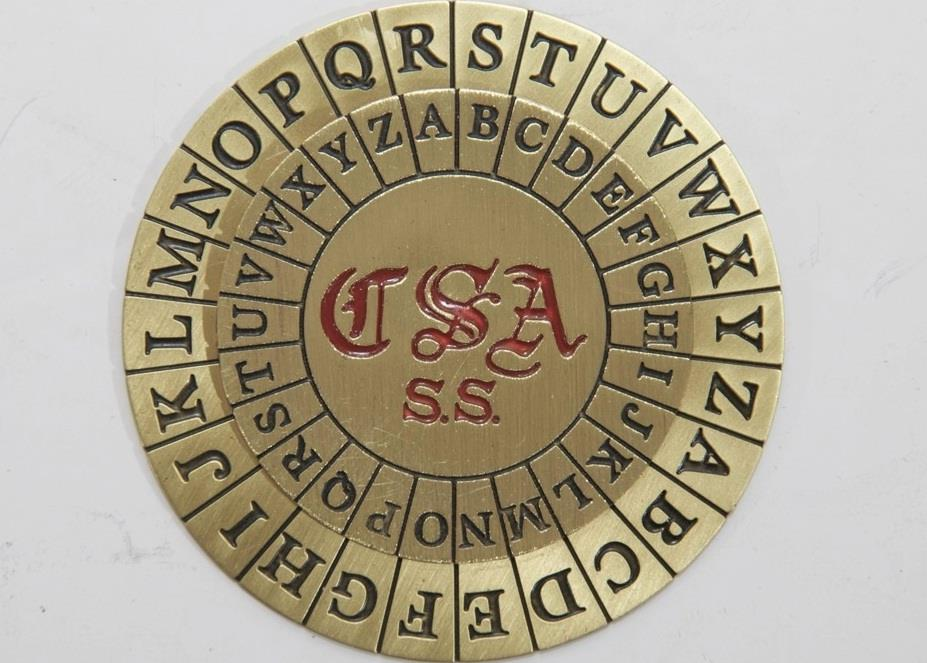
\includegraphics[width=0.85\textwidth]{../../images/python/page_049_img_01.jpeg}

% deskripsi: gambar native xref 243
\noindent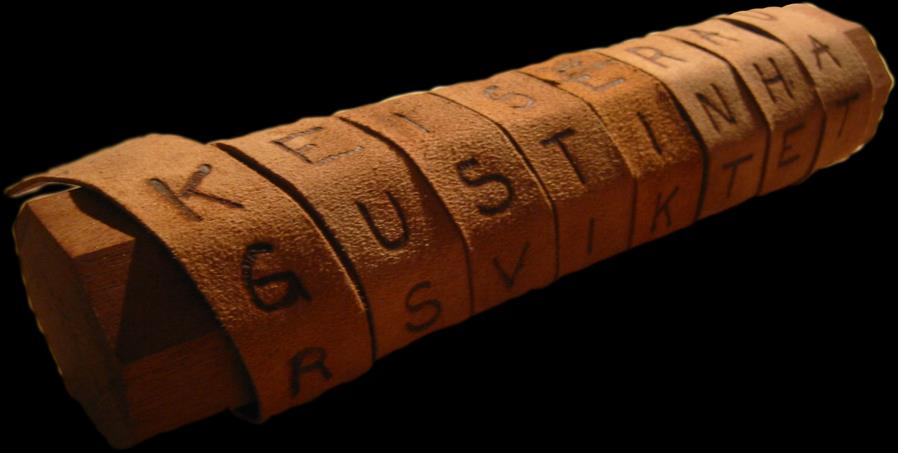
\includegraphics[width=0.85\textwidth]{../../images/python/page_049_img_02.jpeg}

\end{document}
